\documentclass[Main/main.tex]{subfiles}

\begin{document}

\chapter{Theory and Methods}
%SOPs!
%Reasonable level of detail
%Sufficient detail how you have planned and conducted your experimetal work
%Everything needed to understand discussions

%Experimental design, method for synthesis - equqtions and structures
%Instrumentation, analytic methods - SOP, numbers, type of instruments
%Samples, chemicals, materials
%Preparation and storage - commercial source 
%Models and statistical tools

In the following chapter theory regarding electrochemistry, characterization and liquid injection system relevant for the project is presented. 

\section{Electrochemistry}
Electrochemistry relates the flow of electrons to chemical changes, commonly seen in fuel cells and batteries. The movement of electrons from one element to another occurs through a redox reaction, relating an oxidised reactant (Ox) to its reduced compound (red), and the amount of electrons released on reduction ($ne^-$).
$$ Ox + ne^- \iff red $$


A battery consists of one or more interconnected electrochemical cells, each supplying a current ($I$) at a voltage ($V$) for a time $\Delta t$. For a battery to be rechargeable, the redox reaction occuring at the two electrodes need to be reversible.

The electrolyte separating the anode and the cathode may be liquid or solid. Liquid electrolytes are often used with solid electrodes, while a solid electrolyte commonly is in use whith liquid or gaseous electrodes. With a liquid electrolyte, the electrodes are kept apart by an electrolyte-permeable separator. As can be seen from figure \ref{fig:2_jacs}, the electrolyte permits the ionic component of the redox reaction (occuring at the electrodes) to pass through while forcing the electronic component to do work by traversing an external circuit. 

\begin{figure}[ht]
	\centering
	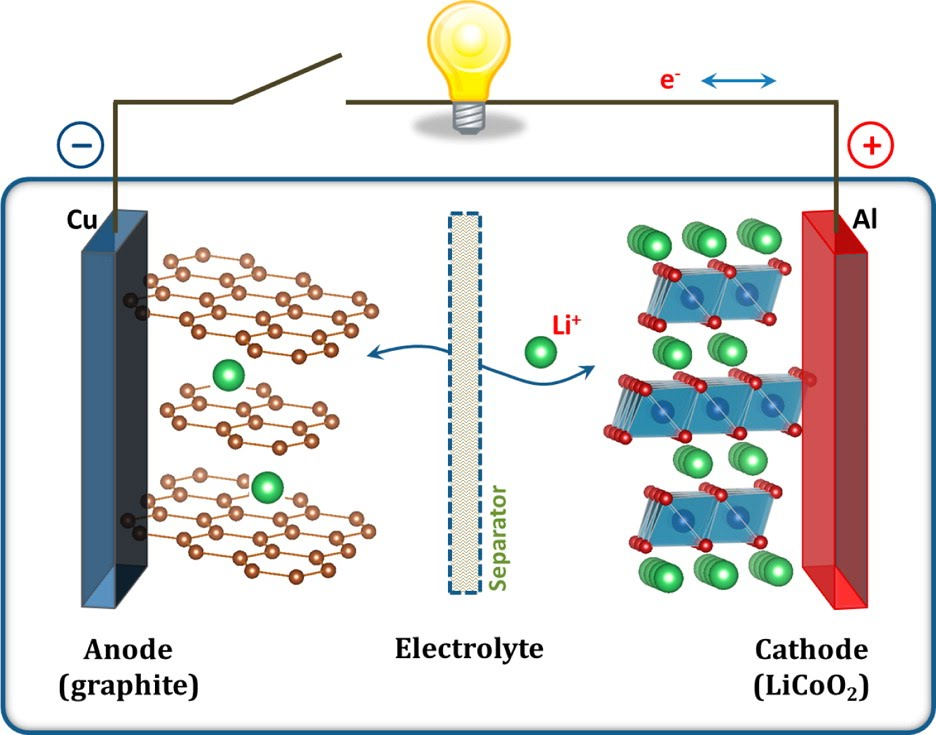
\includegraphics[width=0.7\linewidth]{uploads/JACS}
	\caption{Schematic of the first Li-ion battery. Ions are permitted through the electrolyte while electrons traverse the external circuit.}
	\label{fig:2_jacs}
\end{figure}


$Q(I)$ is the cell capacity for a given current, $I$. $Q$ is the total charge per unit weight (\si{Ah\ kg^{-1}}/\si{mAh\ g^{-1}}) or per volume (\si{Ah\ L^{-1}}). The dependency of $I$ arises since the rate of transfer of ions becomes diffusion-limited at high currents. 

A perfect battery would be able to dispatch the same charge on discharge as it is supplied while charging - every time. In other words, there should ideally not be any capacity fade throughout the life of the battery. A diffusion-limited loss of ions presents a reversible loss of capacity. However, changes in electrode volume, electrode decomposition or chemical reactions between electrode and electrolyte may cause an irreversible loss of capacity \cite{2_Goodenough_perspective}.

The Coloumbic efficiency, \[ 100 \times \frac{Q_{dis}}{Q_{ch}} \] gives the efficiency of a single cycle associated with capacity fade. The cycle life of a battery is the amount of cycles the battery can withstand before the capacity has faded to $80\%$ of its initial reversible value.

Chemical reactions between electrode and electrolyte also leads to the irreversible formation of a passivating solid-electrolyte layer (SEI) on the anode. A SEI is formed during charging and compete with the reversible lithium intercalation \cite{2_SEI}. While a SEI contributes to a capacity fade of the cell, it also enhances the stability and safety of the battery serving as a barrier between the electrode and electrolyte.


\section{Scanning Electron Microscope}
The scanning electron microscope (SEM) scans a focused electron beam over the surface area of a specimen, exploring the microscopic structure with a higher resolution and much greater depth of field compared to an optical microscope. The large depth of field results in a three-dimensional appearance of the resulting images. In addition, chemical information from a specimen can be obtained through the use of various techniques, including using a X-ray energy-dispersive spectrometer (EDS).

A SEM is composed of an electron gun and a series of electromagnetic lenses and apertures as depicted in figure \ref{fig:SEM}. Energetic electrons striking a specimen may be scattered elastically (backscatterd electrons) or inelastically (secondary electrons), or simply pass through without being scattered. Due to difference in energy and angle of the reflected and transmitted electrons, the three types can be measured by different detectors, each providing different types of image production. Figure \ref{fig:SEM} shows the structure of a SEM (left) and the interaction zone of electrons and atoms below a specimen surface (right) indicating the penetration depth of the various electrons. 

\begin{figure}
    \centering
    \includegraphics[width=0.55\textwidth, keepaspectratio]{uploads/SEM-structure}\includegraphics[width=0.45\textwidth, keepaspectratio]{uploads/SEM-droplet}
    \caption{The structure of a SEM (left) \cite{SEM_structure} and the interaction zone where electrons scatter below the specimen surface (right) \cite{SEM_droplet}.}
    \label{fig:SEM}
\end{figure}

\section{X-ray diffraction}
X-rays are a form of electromagnetic radiation with wavelengths ranging from 0.1 to 100 \si{\angstrom}, first discovered by Wilhelm C. Röntgen in 1895. These wavelengths are in the order of interatomic distances in crystals causing diffracted waves to form a unique diffraction pattern due to interference. Thus, X-rays have proven to be an excellent probe of the structure of matter \cite{2_XRD,Scotman}.

The condition for constructive interference is described by Bragg's law as
    $$n\lambda = 2d\sin{\theta}$$
where \textit{n} is an integer, \textit{d} is the lattice spacing, \textit{$\lambda$} is the wavelength of the diffracted beam and \textit{$\theta$} is the diffraction angle. An illustration of the geometry is shown in figure \ref{fig:bragg}.

\begin{figure}[ht]
    \centering
    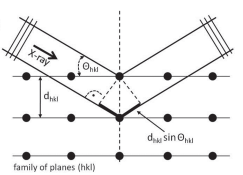
\includegraphics{uploads/Bragg.jpg}
    \caption{Visualization of the principles used to derive Bragg's law \cite{Scotman}.}
    \label{fig:bragg}
\end{figure}

By plotting the counted reflections as a function of the angle between the incident and the diffracted beam (angle of diffraction), the positions and intensities of the peaks function as a fingerprint for the identification of unknown materials by comparing the diffraction pattern with a reference database. Further comprehensive analysis can supply information regarding bond lengths, bond angles, structural disorder and more \cite{Scotman}.



\section{Electrochemical analysis}
When investigating the electrochemical properties of a battery, the cell voltage and the current are often the main parameters of interest. With one of these parameters fixed and the other monitored, valuable information regarding the electrochemical properties can be obtained. The techniques utilised in this thesis are Electric Impedance Spectroscopy (EIS), Cyclic Voltammetry (CV) and Galvanostatic Cycling (GC).

\subsection{Electric Impedance Spectroscopy}
Impedance is a measurement of the opposition a circuit presents to a current, or a change in current, with an applied voltage. Impedance possesses both magnitude and phase and extends the concept of resistance to alternating current (AC) circuits. Thus, impedance is said to be a broadened description of Ohm's law, being a complex value where the real part (Re) is the Ohmic resistance and the imaginary part (Im) represents capacitance and inductance.

To measure the electrochemical impedance a sinusoidal AC-voltage is usually applied to an electrochemical cell and the current signal is measured. By doing this for a range of frequencies one obtains a measured spectrum which can be used to analyse different charge carriers present in the battery. The results from EIS sweeps are often presented in a Nyquist plot, plotting Re(Z) vs. $\pm$ Im(Z).

\begin{comment}
Motstand synker når frekvensen øker. Imaginær - bølger med topper ved størst helling. Nyquist plotter disse to mot hverandre
Frekvensen med høyest respons.
Nedgangen representerer 

Kan si: jevnt over lavere topper - mindre motstand enn høyere topper Totale motstanden
Kan prøve å analysere hva slags ledingsmekanismer man har i batteriet

impedans-responsen til forksjellige ledningsbære ved forskjellige frekvenser
\end{comment}

\subsection{Cyclic voltammetry}
CV is a highly versatile and useful technique commonly employed to investigate the reduction and oxidation properties of a given material. In addition, CV is used to study electron transfer-initiated chemical reactions \cite{2_CV}. During CV, current is measured as a function of applied voltage. With a minimum and maximum voltage set, the measurement starts at zero current voltage (0CV). From there, the voltage is swept at at constant scan rate to the maximum voltage, then to the minimum voltage and ends up at 0CV. This scan is repeated for a number of cycles. Figure \ref{fig:CV} shows a typical CV plot containing the classical "duck" shape. Peaks corresponding to chemical reactions occurring in the battery are present at B and D and the direction of the voltage is changed at C and E.

\begin{figure}[ht]
    \centering
    \includegraphics{uploads/CV_im}
    \caption{A typical cyclic voltammetric profile. The peaks at B and D correspond to chemical reactions occuring in the battery, while C and E is where the applied voltage is reversed \cite{CV_im}.}
    \label{fig:CV}
\end{figure}

\FloatBarrier
\subsection{Galvanostatic cycling}
During GC a constant current is forced into or out of the battery. The cell is cyclically charged and discharged at a constant current between voltage limits defined by the chemistry of the battery and the voltage is recorded as a function of time. Figure \ref{fig:GC} shows the different stages during a measurement.
GC provides insight about the specific capacity, lifetime and cycling stability of the battery cell at different current densities \cite{kvamme}.

\begin{figure}[ht]
    \centering
    \includegraphics[scale=0.9]{uploads/GC}
    \caption{The different stages during a GC measurement \cite{GC}.}
    \label{fig:GC}
\end{figure}


\section{Liquid injection system in vacuum}
The main goal of this thesis is to explore a novel system for the formation of oxides from a variety of more or less complex compounds. The system produces powder that sticks to the surfaces present during synthesis. Liquid is injected in pre-determined amounts (droplets) into a round bottom flask under vacuum and heated. The solvent evaporates and the precursor decomposes into oxides which are then deposited on the substrates present in the flask as well as the surface of the flask itself.

As explained in the introduction, this system is similar to spray pyrolysis with the exception of this process to operate under vacuum. Due to the vacuum, the synthesised oxides adhere surprisingly well to the surfaces present and seems to disperse in the entire chamber, which in this case is a round-bottom flask.

This behaviour can be exploited to synthesize cathodes without the need for a binder in order to have the oxide stick to a conducting surface and will be covered extensively in the following section.


\chapter{Experimental design}

This section intends to give an overview of the instrumentation used in this thesis. Since the deposition technique used is a new method, the level of detail will be more extensive.

\section{Liquid injection system} \label{liquid injection}
The system consisted of a 500 ml single-neck round-bottom flask with a joint size of 29/32 (29 mm wide at the top and 32 mm long) attached to a connector pipe, sealed with a Teflon cone  and silicon grease. A 1/16” stainless steel tube, henceforth called injector tube, went from a 6-port Valco valve through a cap on top of the connector tube, and down to the bottom of the neck of the flask. A vacuum pump was connected to the connector tube in order to reduce the pressure of the flask, and the pressure was monitored with the use of a Pirani gauge. A heating mantle and aluminium foil was used to heat the round-bottom flask to 300-400 $\degree C$ during the injection.

In addition to the injector tube, the 6-ports valve connects a 10 mL syringe containing the precursor, a steel tube forming a loop, an open-end tube and a tube supplying nitrogen gas. The 6-ports valve was used in two different positions, controlled by an Arduino. The first position allowed for the tube to be filled with the precursor. The precursor was mechanically injected from the syringe, and any excess liquid went into a waste beaker from the open-end tube. The second position enabled a nitrogen flow to push the liquid from the tube through the injector tube and into the round-bottom flask. A schematic of the apparatus is presented in figure \ref{fig:ehhh1} where the two positions termed a) and b) are shown with dashed lines representing the active channels for each position. 

Two different vacuum pumps were used due to malfunction of the first pump halfway through the experiments. The first was a rotary vane pump and the second a membrane pump.

During the preparation for new runs a round-bottom flask was washed and dried, 10 mL of the precursor solution measured in the syringe, and all the substrates blown and washed with ethanol before carefully placing them in the flask. A variety of glass, Si and steel plates were utilised. Between the runs, the round-bottom flasks were washed in an acid bath, removing most of the deposited material from the previous run. Any residual material that did not get washed away with either acid or water and a brush were thought not to affect the consecutive run.

\begin{figure}[p]
\centering
%\resizebox{\textwidth-7pt}{!}{
\includegraphics[width=\linewidth, keepaspectratio]{uploads/ehhh2} 
\caption{Schematic of the liquid injection system. The different channels active for the two positions are marked a) and b). }
\label{fig:ehhh1}
\end{figure}



\FloatBarrier
\subsection{Parameter testing}
Since this is a novel system, various parameters have been altered in order to see their effect on the synthesised material. The main parameters of interest have been the position of the tip of the injector-tube, affecting the distance the droplets travel before reaching the surface, and the concentration of the precursor(s). Additionally, the placement of the substrates has been investigated. Figure \ref{fig:tipnplace} shows the tip of the injector tube (left) and a holder fabricated for one steel substrate (right). The holder was utilised, but using a little ethanol to make a steel substrate stick to a glass substrate was found to work just as well.

\begin{figure}[ht]
    \begin{subfigure}{0.5\textwidth}
    \centering
    \includegraphics[width=0.8\textwidth, keepaspectratio]{uploads/injector_tip.jpg}
    \end{subfigure}
    \begin{subfigure}{0.5\textwidth}
    \centering
    \includegraphics[width=1.1\textwidth, keepaspectratio]{uploads/holder2.jpg}
    \end{subfigure}
    \caption{Images of the tip of the injector tube (left) and the holder fabricated to hold one steel substrate (right).}
    \label{fig:tipnplace}
\end{figure}


\subsection{Cathode production}
When the parameters proved satisfactory with respect to the synthesised oxides appearing replicable and providing a good particle distribution through SEM inspection, the parameters were kept constant and two sets of cathode materials were synthesised for the assembly of coin cells, 0.25 M and 2.50 M of cations in the precursor solution, trying to synthesise \ce{MnO2}, LMO and LNMO. This is further explained in section 2.3. Very important during these sets of syntheses was the ability to keep parameters consistent. Straight after synthesis, the system was allowed to cool down while still having an inert atmosphere due to the vacuum. As soon as the vacuum was broken, the steel substrates were weighed and moved to a glove box awaiting coin cell assembly. 

The setup used, later termed setup A, is shown in figure \ref{fig:placement}. The setup referred to as setup B is similar, except for the bottom steel substrate placed beneath the topmost glass, just lying on the substrate holder. This did not have any visible effect and setup A was resumed.


\begin{figure}[ht]
    \centering
    \includegraphics[width=0.45\textwidth, keepaspectratio]{uploads/placement_flask.jpg}
    \caption{Image of setup A.}
    \label{fig:placement}
\end{figure}


\section{Precursors}

Metal nitrates (hydrates) are popular precursor components for the preparation of oxides, and their decomposition is well documented \cite{DecompMn,thermal_li, DecompNi}.

\subsection{Chemicals}
All chemicals were used without any further purification and stored as advised by manufacturer. Table \ref{tab:chemicals} shows the chemicals with specifications.

\begin{table}[ht]
	\centering
	\caption{The compounds used as precursors.}
	\label{tab:chemicals}
	\resizebox{\textwidth}{!}{
		\begin{tabular}{cccccc}
			\hline 
			\textbf{Compound} & \textbf{Linear formula} & \textbf{Purity} & \textbf{Supplier} & \textbf{CAS} & \textbf{Lot \#} \\ 
			\hline 
			Manganese(II) nitrate hydrate  & \ce{Mn(NO3)2.5H2O} & 98\% & Sigma-Aldrich & 15710-66-4 & MKBR0853V \\
			
			Manganese(II) nitrate hydrate* & \ce{Mn(NO3)2.4H2O} & Unknown & Unknown & Unknown & Unknown\\
			
			Lithium nitrate & \ce{LiNO3} & $>$ 99\% & Sigma-Aldrich &  7790-69-4 & BCBG3251V \\ 
			
			Nickel(II) nitrate hydrate & \ce{Ni(NO3)2.6H2O} & Unknown & KEBO & 9650672 & 6721 \\ 
			\hline 
		\end{tabular} }
	    \vspace{1ex} \scriptsize{\raggedright{*Due to shortage of the Manganese(II) nitrate hydrate from Sigma-Aldrich, an old batch found in a closet was used for the last set of runs.}}
	\end{table}


\subsubsection{Stochiometry}

In order to verify the stochiometry of the synthesised oxides, 1mL of the prepared solution was measured into a weighed glass vial, left in a oven at 60 \degree C until most of the solvent had evaporated, and then placed in a furnace holding 400 \degree C for a couple minutes until the nitrates had decomposed into oxides. A new weighing of the glass vial supplied the mass of the synthesised oxide, making it possible to calculate the stochiometry required for the number of moles of the precursor(s) to match the number of moles of the synthesised oxide. This approach was also used to verify the degree of hydration for the two \ce{Mn(NO3)2.xH2O} used.



\section{Experimental runs}
The water used as solvent was ASTM type II water. The concentration of cations in the precursors will be used to distinguish the different oxides.

\paragraph{\ce{MnO2}}~\\
For the first set of testing, 12 mmol of \ce{Mn(NO3)2.5H2O} was dissolved in water and diluted to a concentration of 0.120 M. The solution was mixed well and used in the synthesis as explained in section \ref{liquid injection}.

To make a solution of increased concentration, 12.6 mmol of \ce{Mn(NO3)2.5H2O} was dissolved in 50 mL water, yielding a concentration of 0.252 M. 

For the further ten-fold increase in concentration, the Manganese(II) nitrate hydrate marked with an asterix in table \ref{tab:chemicals} was used. 62.52 mmol of \ce{Mn(NO3)2.4H2O} was dissolved in 25 mL water, yielding a concentration of 2.50 M.


\paragraph{LMO}~\\
In order to synthesise LMO, \ce{LiNO3} and \ce{Mn(NO3)2.5H2O} were weighed out to obtain the molar ratio of metal components (Li:Mn) of 1:2 and dissolved to prepare aqueous solutions of 0.252 and 2.5 M. (4.2 [20.83] mmol \ce{LiNO3} and 8.39 [41.67] mmol \ce{Mn(NO3)2.5H2O} were dissolved separately and mixed to a solution of 50 [25] mL).

\paragraph{LNMO}~\\
To synthesise LNMO, \ce{LiNO3}, \ce{Ni(NO3)2.6H2O} and \ce{Mn(NO3)2.5H2O} were weighed out to obtain the molar ratio of metal components (Li:Ni:Mn) of 1:0.5:1.5 and dissolved to prepare aqueous solutions of 0.252 and 2.5M. (4.20 [20.85] mmol \ce{LiNO3}, 2.10 [10.41] mmol \ce{Ni(NO3)2.6H2O} and 6.31 [31.24] mmol \ce{Mn(NO3)2.5H2O} were dissolved separately and mixed to a solution of 50 [25] mL).



\begin{table}[ht]
    \caption{Table of the different runs conducted.}
    \label{tab:runs}
	\resizebox{\textwidth}{!}{
\begin{tabular}{c c c c c}
	\toprule
	Experiment & Concentration of cations & Precursor(s) & Substrates & Notice \\ 
	\midrule
	\multicolumn{5}{c}{Testing parameters} \\[1em]
    
	01 & 0.120 M & \ce{Mn} & 1x Glass, 1x Si  & First run  \\ 
	
	02 & 0.120 M & \ce{Mn} & 1x Glass, 1x Si & Duplicate of experiment 01 \\ 
	
	03 & 0.120 M & \ce{Mn} & 1x Glass, 1x Si & Injector wire 1 cm up from run 001 \\ 
	
	04 & 0.120 M & \ce{Mn} & 1x Glass, 1x Si & Injector wire 1 cm down from run 001 \\
	
	05 & 0.120 M & \ce{Mn} & 1x Glass & Injector wire 2 cm down from run 001 \\
	
	06 & 0.120 M & \ce{Mn} & 1x Glass, 1x Steel & Steel plate positioned below glass \\ 
	
	07 & 0.120 M & \ce{Mn} & 1x Glass, 1x Steel & Steel plate positioned above glass \\
	
	08 & 0.120 M & \ce{Mn} & 1x Steel & Sample holder hung vertically from the wire \\ 
	
    09 & 0.120 M & \ce{Mn} & 1x Glass, 1x Steel & Sample holder adjusted \\ 
	
	10 & 0.252 M & \ce{Mn} & 1x Glass, 1x Steel & Sample holder placed horizontally. Injector wire changed \\ 

	11 & 0.252 M & \ce{Mn} & 1x Glass, 1x Steel & Duplicate of experiment 10\\ 
	
	12 & 0.252 M & \ce{Mn} & 1x Glass, 1x Steel & Duplicate of experiment 10\\
	\hline 
	\multicolumn{5}{c}{Setup fixed} \\[1em]
	
	13 & 0.252 M & \ce{Li, Mn} & 2x Glass, 3x Steel & Setup A \\ 
	
	14 & 0.252 M & \ce{Li, Mn} & 2x Glass, 2x Steel & Setup A \\ 
	
	15 & 0.252 M & \ce{Li, Mn} & 3x Glass, 3x Steel & Setup B \\ 
	
	16 & 0.252 M & \ce{Li, Mn} & 3x Glass, 1x Si, 2x Steel & Setup A \\ 
	
	17 & 0.252 M & \ce{Li, Mn} & 3x Glass, 1x Si, 2x Steel & Setup A \\ 
	
	18 & 0.252 M & \ce{Li, Ni, Mn} & 3x Glass, 1x Si, 2x Steel & Setup A \\ 
	
	19 & 0.252 M & \ce{Li, Ni, Mn} & 3x Glass, 1x Si, 2x Steel & Setup A \\ 
	
	20 & 0.252 M & \ce{Li, Mn} & 3x Glass, 3x Steel & Setup A \\
	
	21 & 0.252 M & \ce{Li, Mn} & 3x Glass, 3x Steel & Setup A \\
	
	22 & 2.50 M & \ce{Li, Mn} & 3x Glass, 3x Steel & Setup A \\
	
	23 & 2.50 M & \ce{Mn} & 3x Glass, 3x Steel & Setup A \\
	
	24 & 2.50 M & \ce{Li, Ni, Mn} & 3x Glass, 3x Steel & Setup A. Discarded \\
	
	25 & 2.50 M & \ce{Li, Ni, Mn} & 3x Glass, 3x Steel & Setup A \\ 
	\bottomrule
\end{tabular} }
\end{table}

\section{X-ray diffraction}
X-ray diffraction was performed with a Bruker AXS D8 discover diffractometer in reflection mode. The XRD data was analysed with DIFFRAC.EVA from Bruker.

\section{Scanning electron microscopy}
Scanning electron microscopy was performed on a tabletop Hitachi TM3000 operating at 5kV, equipped with a Silicon drift EDS detector and a thermionic emission cannon using a tungsten filament.

%operert med programvare TM3000 versjon 02-03-02. Quantax 70 - 2010


\section{Coin-Cell Assembly}
To investigate the electrochemical properties of the synthesised cathodes, CR2032 coin cells were built using metallic lithium as the anode and the as-deposited steel plates as cathodes. The cells were assembled inside an MBraun Labmaster glovebox with argon atmosphere, and water and oxygen levels below 0.1ppm. A Whatman glass microfiber sheet was used as the separator membrane and the liquid electrolyte consisted of 1M $\chemfig{LiClO_4}$ in a 1:1 mixture of ethyl carbonate (EC) and dimethyl carbonate (DMC).

\section{Electrochemical analysis}
Cycling voltammetry and Galvanostatic cycling was performed on a MPG2 probostat from BioLogic using EC-Lab software. Impedance spectroscopy was performed on a VSP potentiostat from BioLogic, also using EC-lab software. The data from all measurements was treated in Origin and the results are presented in the following section.


\end{document}